% file: 3-9-connectivity/2conn-adjacent-edges.tex

\documentclass[tikz]{standalone}
\usetikzlibrary{positioning, decorations.pathmorphing}

\begin{document}
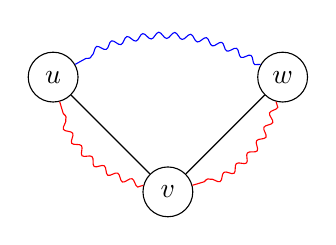
\begin{tikzpicture}[every node/.style = {draw, circle, minimum size = 18pt},
    path/.style = {-, decorate, decoration = {snake, amplitude = .4mm, segment length = 2mm, post length = 1mm}}]
  \node (v) {$v$};
  \node (u) [above left = of v] {$u$};
  \node (w) [above right = of v] {$w$};

  \path (v) edge (u)
  	    edge (w)
	(w) edge[blue, bend right, path] (u)
	    edge[red, bend left, path] (v)
	(v) edge[red, bend left, path] (u);
\end{tikzpicture}
\end{document}